\section{Architettura Back-End} \label{sec:archback}

Coerentemente alla struttura imposta dall'adozione di una Clean Architecture, il back-end dell'applicazione è organizzato tramite delle classi controller, use case, repository e data source.\\
Per collegare l'interfaccia grafica lato front-end con il funzionamento dell'applicativo lato back-end, sono state implementate delle server actions per chiamare i controller relativi all'azione desiderata.\\
I controller eseguono la chiamata allo use case relativo, che costituisce ed implementa la business logic dell'intero sistema.\\
Per accedere alle fonti dei dati, necessari a realizzare le funzionalità definite dai casi d'uso, le classi use cases si relazionano con delle classi repositories, nelle quali è posta la logica di persistenza, che presentano i metodi per lettura, scrittura ed eliminazione dei dati.\\
La singola classe repository si interfaccia alla classe data source ad essa associata, la quale presenta i metodi che intervengono concretamente sulle fonti dei dati per compiere le funzioni richieste sui database.\\
Una volta terminate le operazioni nel data source, il controllo torna alla repository, la quale ritorna i dati recuperati allo use case quando richiesto. Completata la funzionalità definita dal caso d'uso, il flusso di controllo torna al controller che dovrà gestire la risposta verso la server action da cui tutto è iniziato.

\begin{figure}[h!]
    \centering  
    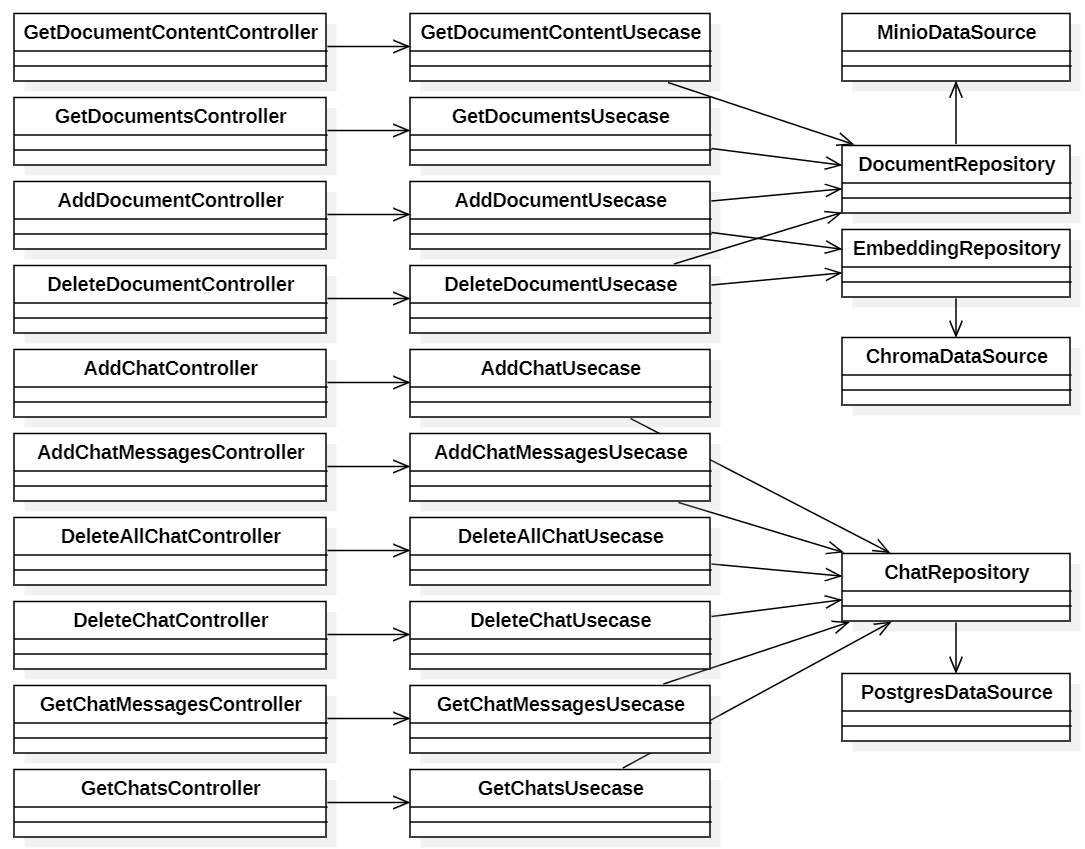
\includegraphics[width=0.7\textwidth]{backendview.png}
    \caption{UML introduttivo delle classi del back-end}
\end{figure}

\newpage


\subsection{Server Actions} \label{subsec:serveractions}

\subsubsection{addDocument}
\textbf{Parametri}
\begin{itemize}
    \item \textit{data: FormData}.
\end{itemize}
\textbf{Descrizione}\\
Questa funzione asincrona lato server effettua una chiamata a AddDocumentController, passando il parametro data. Data contiene una \textit{string} model e un \textit{File} file, che rappresentano il modello che deve presentare il nuovo documento e il file da aggiungere. Gestisce l'aggiunta di un documento inviando i dati al controller e si occupa di gestire eventuali errori che si possono verificare durante il processo.


\subsubsection{deleteDocument}
\textbf{Parametri}
\begin{itemize}[itemsep=-4pt]
    \item \textit{name: string};
    \item \textit{model: IModel}.
\end{itemize}
\textbf{Descrizione}\\
Questa funzione asincrona lato server effettua una chiamata a DeleteDocumentController, passando i parametri name e model, che rappresentano il nome del documento da eliminare e il modello che non deve più presentare tale documento. Gestisce l'eliminazione di un documento inviando i dati al controller e si occupa di gestire eventuali errori che si possono verificare durante il processo.

\subsubsection{getDocument}
\textbf{Parametri}
\begin{itemize}
    \item \textit{model: IModel}.
\end{itemize}
\textbf{Descrizione}\\
Questa funzione asincrona lato server effettua una chiamata a GetDocumentsController, passando il parametro model, che rappresenta il modello da cui prendere i documenti associati. Gestisce il recupero delle informazioni dei documenti inviando i dati al controller e si occupa di gestire eventuali errori che si possono verificare durante il processo.

\subsubsection{getDocumentContent}
\textbf{Parametri}
\begin{itemize}[itemsep=-4pt]
    \item \textit{docName: string};
    \item \textit{model: IModel}.
\end{itemize}
\textbf{Descrizione}\\
Questa funzione asincrona lato server effettua una chiamata a GetDocumentContentController, passando i parametri docName e model, che rappresentano il nome del documento da cui recuperare il link per la visualizzazione e il modello che presenta tale documento. Gestisce il recupero dell'informazione inviando i dati al controller e si occupa di gestire eventuali errori che si possono verificare durante il processo.

\subsubsection{updateDocument}
\textbf{Parametri}
\begin{itemize}[itemsep=-4pt]
    \item \textit{docName: string};
    \item \textit{model: IModel};
    \item \textit{visibility: boolean}.
\end{itemize}
\textbf{Descrizione}\\
Questa funzione asincrona lato server effettua una chiamata a UpdateDocumentController, passando i parametri docName, model e visibility, che rappresentano il nome del documento da aggiornare, il modello che presenta tale documento e il nuovo valore che deve avere il tag di visibilità del documento. Gestisce la modifica delle informazioni inviando i dati al controller e si occupa di gestire eventuali errori che si possono verificare durante il processo.

\subsubsection{addChat}
\textbf{Parametri}
\begin{itemize}
    \item \textit{title: string}.
\end{itemize}
\textbf{Descrizione}\\
Questa funzione asincrona lato server effettua una chiamata a AddChatController, passando il parametro title, che rappresenta il nome della sessione di conversazione da aggiungere. Gestisce la creazione della sessione inviando i dati al controller e si occupa di gestire eventuali errori che si possono verificare durante il processo.

\subsubsection{addChatMessages}
\textbf{Parametri}
\begin{itemize}
    \item \textit{messages: ICustomMessages}.
\end{itemize}
\textbf{Descrizione}\\
Questa funzione asincrona lato server effettua una chiamata a AddChatMessagesController, passando il parametro messages, che rappresenta il messaggio da salvare relativo ad una sessione di conversazione. Gestisce il salvataggio del messaggio inviando il dato al controller e si occupa di gestire eventuali errori che si possono verificare durante il processo.

\subsubsection{deleteAllChat}
\textbf{Descrizione}\\
Questa funzione asincrona lato server effettua una chiamata a DeleteAllChatController per eliminare tutti i dati relativi a sessioni e chat history. Gestisce l'eliminazione di queste informazioni effettuando una chiamata al controller e si occupa di gestire eventuali errori che si possono verificare durante il processo.

\subsubsection{deleteChat}
\textbf{Parametri}
\begin{itemize}
    \item \textit{id: number}.
\end{itemize}
\textbf{Descrizione}\\
Questa funzione asincrona lato server effettua una chiamata a DeleteChatController, passando il parametro id, che rappresenta il valore univoco della sessione di conversazione da eliminare. Gestisce l'eliminazione della sessione inviando i dati al controller e si occupa di gestire eventuali errori che si possono verificare durante il processo.

\subsubsection{getChatMessages}
\textbf{Parametri}
\begin{itemize}
    \item \textit{id: number}.
\end{itemize}
\textbf{Descrizione}\\
Questa funzione asincrona lato server effettua una chiamata a GetChatMessagesController, passando il parametro id, che rappresenta il valore univoco della sessione di conversazione da cui recuperare la chat history. Gestisce il recupero dati della sessione inviando il parametro al controller e si occupa di gestire eventuali errori che si possono verificare durante il processo.

\subsubsection{getChats}
\textbf{Descrizione}\\
Questa funzione asincrona lato server effettua una chiamata a GetChatsController, con cui recupera le informazioni delle sessioni di conversazione attive nell'applicazione. Gestisce il recupero dati delle sessioni ed eventuali errori che si possono verificare durante il processo.

\newpage

\subsection{Controllers} \label{subsec:controllers}
\subsubsection{AddDocumentController}
\textbf{Decoratori}
\begin{itemize}
    \item \textit{@injectable()}: decoratore per la Dependency Injection mediante Tsyringe.
\end{itemize}
\textbf{Attributi}
\begin{itemize}
    \item private readonly \textit{\_useCase: AddDocumentUsecase}.
\end{itemize}
\textbf{Metodi}
\begin{itemize}
    \item \textit{handle(data: FormData): Promise<Response>}.
\end{itemize}
\textbf{Descrizione}\\
Questa classe controller, chiamata tramite la server action addDocument, gestisce la chiamata al AddDocumentUsecase per aggiungere a sistema un nuovo documento, passando un \textit{FormData} contenente una \textit{string} model e un \textit{File} file, che rappresentano il modello che deve presentare il nuovo documento e il file da aggiungere.\\ \\
\textbf{Dipendenze}
\begin{itemize}
    \item AddDocumentUsecase.
\end{itemize}

\begin{figure}[h!]
    \centering  
    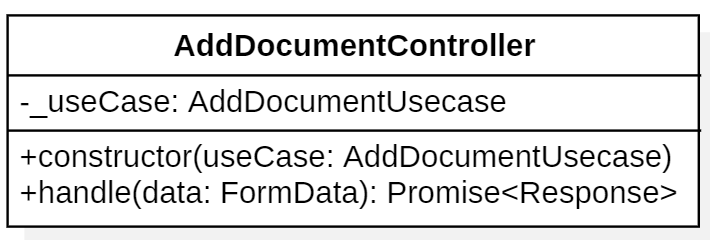
\includegraphics[width=0.5\textwidth]{AddDocumentController.png}
    \caption{UML della classe AddDocumentController}
\end{figure}

\subsubsection{DeleteDocumentController}
\textbf{Decoratori}
\begin{itemize}
    \item \textit{@injectable()}: decoratore per la Dependency Injection mediante Tsyringe.
\end{itemize}
\textbf{Attributi}
\begin{itemize}
    \item private readonly \textit{\_useCase: DeleteDocumentUsecase}.
\end{itemize}
\textbf{Metodi}
\begin{itemize}
    \item \textit{handle(docName: string, model: IModel): Promise<Response>}.
\end{itemize}
\textbf{Descrizione}\\
Questa classe controller, chiamata tramite la server action deleteDocument, gestisce la chiamata al DeleteDocumentUsecase per eliminare dal sistema un documento, passando una \textit{string} docName e una \textit{string} model, che rappresentano il nome del documento da eliminare e il modello da cui rimuoverlo.\\ \\
\textbf{Dipendenze}
\begin{itemize}
    \item DeleteDocumentUsecase.
\end{itemize}

\begin{figure}[h!]
    \centering  
    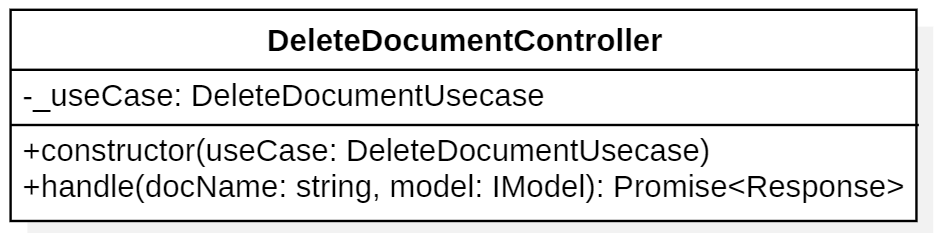
\includegraphics[width=0.6\textwidth]{DeleteDocumentController.png}
    \caption{UML della classe DeleteDocumentController}
\end{figure}

\subsubsection{UpdateDocumentController}
\textbf{Decoratori}
\begin{itemize}
    \item \textit{@injectable()}: decoratore per la Dependency Injection mediante Tsyringe.
\end{itemize}
\textbf{Attributi}
\begin{itemize}
    \item private readonly \textit{\_useCase: UpdateDocumentUsecase}.
\end{itemize}
\textbf{Metodi}
\begin{itemize}
    \item \textit{handle(docName: string, model: IModel, visibility: boolean): Promise<Response>}.
\end{itemize}
\textbf{Descrizione}\\
Questa classe controller, chiamata tramite la server action updateDocument, gestisce la chiamata al UpdateDocumentUsecase per aggiornare i tag e i metadati associati ad un documento, passando una \textit{string} docName, una \textit{string} model e un \textit{booleano} visibility, che rappresentano il nome del documento da aggiornare, il modello di appartenenza e il nuovo valore del tag di visibilità associato.\\ \\
\textbf{Dipendenze}
\begin{itemize}
    \item UpdateDocumentUsecase.
\end{itemize}

\begin{figure}[h!]
    \centering  
    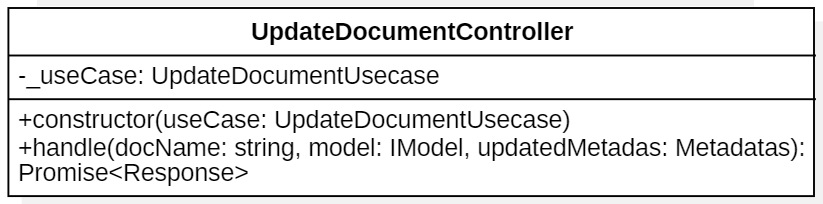
\includegraphics[width=0.7\textwidth]{UpdateDocumentController.png}
    \caption{UML della classe UpdateDocumentController}
\end{figure}

\subsubsection{GetDocumentContentController}
\textbf{Decoratori}
\begin{itemize}
    \item \textit{@injectable()}: decoratore per la Dependency Injection mediante Tsyringe.
\end{itemize}
\textbf{Attributi}
\begin{itemize}
    \item private readonly \textit{\_useCase: GetDocumentContentUsecase}.
\end{itemize}
\textbf{Metodi}
\begin{itemize}
    \item \textit{handle(docName: string, model: IModel): Promise<Response>}.
\end{itemize}
\textbf{Descrizione}\\
Questa classe controller, chiamata tramite la server action getDocumentContent, gestisce la chiamata al GetDocumentContentUsecase per recuperare dal sistema il link di visualizzazione di un documento, passando una \textit{string} docName e un \textit{IModel} (stringa con il nome di un modello) model, che rappresentano il nome del documento di interesse e il modello che presenta il documento.\\ \\
\textbf{Dipendenze}
\begin{itemize}
    \item GetDocumentContentUsecase.
\end{itemize}

\begin{figure}[h!]
    \centering  
    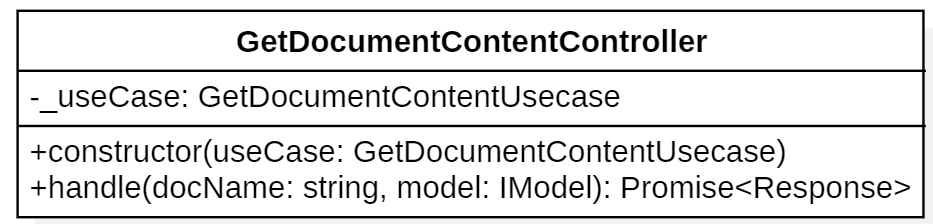
\includegraphics[width=0.6\textwidth]{GetDocumentContentController.png}
    \caption{UML della classe GetDocumentContentController}
\end{figure}

\subsubsection{GetDocumentsController}
\textbf{Decoratori}
\begin{itemize}
    \item \textit{@injectable()}: decoratore per la Dependency Injection mediante Tsyringe.
\end{itemize}
\textbf{Attributi}
\begin{itemize}
    \item private readonly \textit{\_useCase: GetDocumentsUsecase}.
\end{itemize}
\textbf{Metodi}
\begin{itemize}
    \item \textit{handle(model: IModel): Promise<Response>}.
\end{itemize}
\textbf{Descrizione}\\
Questa classe controller, chiamata tramite la server action getDocuments, gestisce la chiamata al GetDocumentsUsecase per recuperare le informazioni dei documenti quali nome, data di ultima modifica e dimensione, passando una \textit{string} model, che rappresenta il nome del modello da cui recuperare i documenti.\\ \\
\textbf{Dipendenze}
\begin{itemize}
    \item GetDocumentsUsecase.
\end{itemize}

\begin{figure}[h!]
    \centering  
    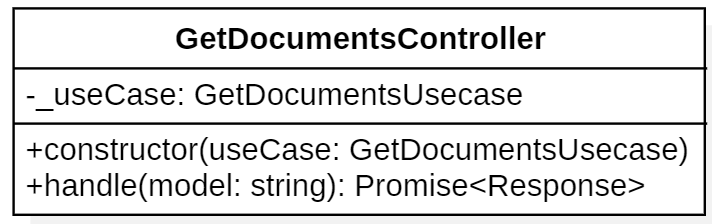
\includegraphics[width=0.6\textwidth]{GetDocumentsController.png}
    \caption{UML della classe GetDocumentsController}
\end{figure}

\subsubsection{AddChatController}
\textbf{Decoratori}
\begin{itemize}
    \item \textit{@injectable()}: decoratore per la Dependency Injection mediante Tsyringe.
\end{itemize}
\textbf{Attributi}
\begin{itemize}
    \item private readonly \textit{\_useCase: AddChatUsecase}.
\end{itemize}
\textbf{Metodi}
\begin{itemize}
    \item \textit{handle(title: string): Promise<Response>}.
\end{itemize}
\textbf{Descrizione}\\
Questa classe controller, chiamata tramite la server action addChat, gestisce la chiamata al AddChatUsecase per creare una nuova sessione di conversazione, passando una \textit{string} title che rappresenta il nome che prenderà quella sessione.\\ \\
\textbf{Dipendenze}
\begin{itemize}
    \item AddChatUsecase.
\end{itemize}

\begin{figure}[h!]
    \centering  
    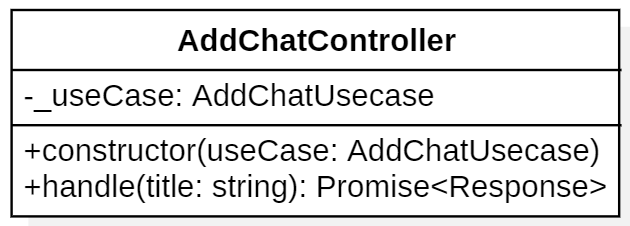
\includegraphics[width=0.6\textwidth]{AddChatController.png}
    \caption{UML della classe AddChatController}
\end{figure}

\subsubsection{AddChatMessagesController}
\textbf{Decoratori}
\begin{itemize}
    \item \textit{@injectable()}: decoratore per la Dependency Injection mediante Tsyringe.
\end{itemize}
\textbf{Attributi}
\begin{itemize}
    \item private readonly \textit{\_useCase: AddChatMessagesUsecase}.
\end{itemize}
\textbf{Metodi}
\begin{itemize}
    \item \textit{handle(messages: ICustomMessages): Promise<Response>}.
\end{itemize}
\textbf{Descrizione}\\
Questa classe controller, chiamata tramite la server action addChatMessages, gestisce la chiamata al AddChatMessagesUsecase dove viene passato un nuovo messaggio scambiato in una sessione (messages: \textit{ICustomMessages}) da aggiungere nel database.\\ \\
\textbf{Dipendenze}
\begin{itemize}
    \item AddChatMesagesUsecase.
\end{itemize}

\begin{figure}[h!]
    \centering  
    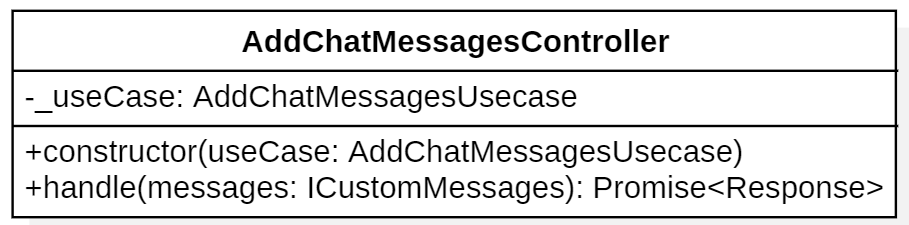
\includegraphics[width=0.6\textwidth]{AddChatMessagesController.png}
    \caption{UML della classe AddChatMessagesController}
\end{figure}

\subsubsection{DeleteAllChatController}
\textbf{Decoratori}
\begin{itemize}
    \item \textit{@injectable()}: decoratore per la Dependency Injection mediante Tsyringe.
\end{itemize}
\textbf{Attributi}
\begin{itemize}
    \item private readonly \textit{\_useCase: DeleteAllChatUsecase}.
\end{itemize}
\textbf{Metodi}
\begin{itemize}
    \item \textit{handle(): Promise<Response>}.
\end{itemize}
\textbf{Descrizione}\\
Questa classe controller, chiamata tramite la server action deleteAllChat, gestisce la chiamata al DeleteAllChatUsecase per rimuovere nel database tutte le sessioni e le chat history relative.\\ \\
\textbf{Dipendenze}
\begin{itemize}
    \item DeleteAllChatUsecase.
\end{itemize}

\begin{figure}[h!]
    \centering  
    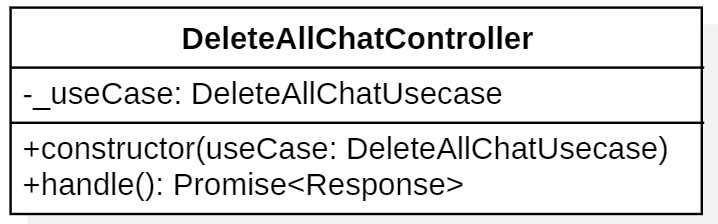
\includegraphics[width=0.6\textwidth]{DeleteAllChatController.png}
    \caption{UML della classe DeleteAllChatController}
\end{figure}

\subsubsection{DeleteChatController}
\textbf{Decoratori}
\begin{itemize}
    \item \textit{@injectable()}: decoratore per la Dependency Injection mediante Tsyringe.
\end{itemize}
\textbf{Attributi}
\begin{itemize}
    \item private readonly \textit{\_useCase: DeleteChatUsecase}.
\end{itemize}
\textbf{Metodi}
\begin{itemize}
    \item \textit{handle(id: number): Promise<Response>}.
\end{itemize}
\textbf{Descrizione}\\
Questa classe controller, chiamata tramite la server action deleteChat, gestisce la chiamata al DeleteChatUsecase per rimuovere dal database una particolare sessione, identificata dal \textit{number} id, e la chat history relativa.\\ \\
\textbf{Dipendenze}
\begin{itemize}
    \item DeleteChatUsecase.
\end{itemize}

\begin{figure}[h!]
    \centering  
    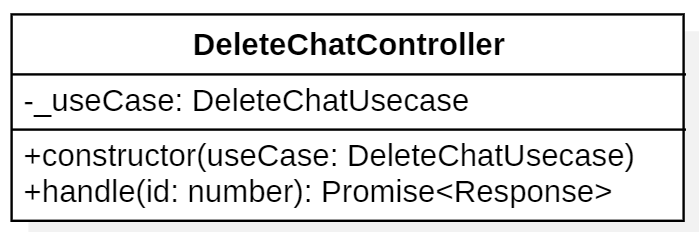
\includegraphics[width=0.6\textwidth]{DeleteChatController.png}
    \caption{UML della classe DeleteChatController}
\end{figure}

\subsubsection{GetChatMessagesController}
\textbf{Decoratori}
\begin{itemize}
    \item \textit{@injectable()}: decoratore per la Dependency Injection mediante Tsyringe.
\end{itemize}
\textbf{Attributi}
\begin{itemize}
    \item private readonly \textit{\_useCase: GetChatMessagesUsecase}.
\end{itemize}
\textbf{Metodi}
\begin{itemize}
    \item \textit{handle(id: number): Promise<Response>}.
\end{itemize}
\textbf{Descrizione}\\
Questa classe controller, chiamata tramite la server action getChatMessages, gestisce la chiamata al GetChatMessagesUsecase per recuperare dal database la chat history di una particolare sessione, identificata dal \textit{number} id.\\ \\
\textbf{Dipendenze}
\begin{itemize}
    \item GetChatMessagesUsecase.
\end{itemize}

\begin{figure}[h!]
    \centering  
    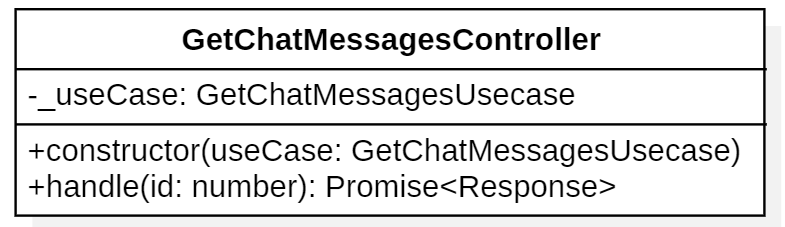
\includegraphics[width=0.6\textwidth]{GetChatMessagesController.png}
    \caption{UML della classe GetChatMessagesController}
\end{figure}

\subsubsection{GetChatsController}
\textbf{Decoratori}
\begin{itemize}
    \item \textit{@injectable()}: decoratore per la Dependency Injection mediante Tsyringe.
\end{itemize}
\textbf{Attributi}
\begin{itemize}
    \item private readonly \textit{\_useCase: GetChatsUsecase}.
\end{itemize}
\textbf{Metodi}
\begin{itemize}
    \item \textit{handle(): Promise<Response}>.
\end{itemize}
\textbf{Descrizione}\\
Questa classe controller, chiamata tramite la server action getChats, gestisce la chiamata al GetChatsUsecase per recuperare dal database le sessioni di conversazione attive nel sistema.\\ \\
\textbf{Dipendenze}
\begin{itemize}
    \item GetChatsUsecase.
\end{itemize}

\begin{figure}[h!]
    \centering  
    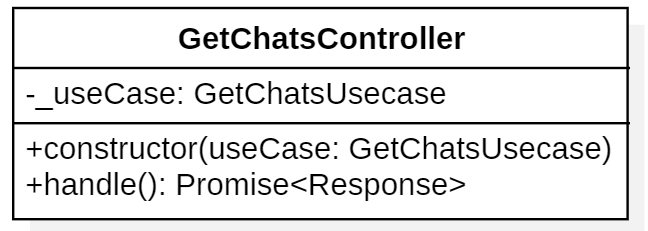
\includegraphics[width=0.6\textwidth]{GetChatsController.png}
    \caption{UML della classe GetChatsController}
\end{figure}

\newpage
